\documentclass[conference]{IEEEtran}

\ifCLASSINFOpdf
  \usepackage[pdftex]{graphicx}
  % declare the path(s) where your graphic files are
  \graphicspath{{images/}}
  % and their extensions so you won't have to specify these with
  % every instance of \includegraphics
  \DeclareGraphicsExtensions{.pdf,.jpeg,.png}
\else
  % or other class option (dvipsone, dvipdf, if not using dvips). graphicx
  % will default to the driver specified in the system graphics.cfg if no
  % driver is specified.
  \usepackage[dvips]{graphicx}
  % declare the path(s) where your graphic files are
  \graphicspath{{../eps/}}
  % and their extensions so you won't have to specify these with
  % every instance of \includegraphics
  \DeclareGraphicsExtensions{.eps}
\fi

\usepackage{stfloats}

\usepackage[cmex10]{amsmath}

\usepackage{algorithmic}

\usepackage{array}

\usepackage[caption=false,font=footnotesize]{subfig}

\usepackage{url}

% Variable for our algorithms to use.
\def \algorithmsToUse {Agglomerative, HDBSCAN*, K-Means++, and K-Medoids}

% correct bad hyphenation here
\hyphenation{op-tical net-works semi-conduc-tor}

\usepackage{amsfonts}

\begin{document}
\title{SDSS MOC4 Asteroids' Color Classifications}


% author names and affiliations
% use a multiple column layout for up to three different
% affiliations
\author{\IEEEauthorblockN{Benjamin Montgomery}
\IEEEauthorblockA{Department of Computer Science\\
University of Southern Maine\\
Portland, Maine 04104\\
Email: benjamin.montgomery@maine.edu}
}

% conference papers do not typically use \thanks and this command
% is locked out in conference mode. If really needed, such as for
% the acknowledgment of grants, issue a \IEEEoverridecommandlockouts
% after \documentclass

% use for special paper notices
%\IEEEspecialpapernotice{(Invited Paper)}


% make the title area
\maketitle

% As a general rule, do not put math, special symbols or citations
% in the abstract
\begin{abstract}
The range of taxonomic categories of asteroids found to be present in the Sloan Digital Sky Survey (SDSS) has varied markedly within the span of a decade, bringing to question the particular methods used by machine learning algorithms to analyze and classify this data. We used the \algorithmsToUse  \, clustering algorithms to attempt to independently verify the methods used by previous papers, finding that some previous classification efforts are not functions of color clusters.
\end{abstract}

\IEEEpeerreviewmaketitle

\section{Introduction}
The Sloan Digital Sky Survey is a multi-spectral survey of celestial objects, most notably of asteroids.
Multiple efforts \cite{chapman_classification, zappal_clustering, Carvano, Autoclass} have been presented to classify these asteroids based on their observed spectra and colors; the expected number of classes existent in the data ranges from two classes \cite{Autoclass} to sixteen \cite{Carvano}.
These analyses fail to capture the accepted twenty-six \cite{binzel_classification} classes found using other asteroid spectral datasets.
The variance appears largely due to the kind of classification methods used; original attempts were made using unsupervised clustering algorithms \cite{zappal_clustering, Carvano}, whereas later efforts were supervised learning algorithms that relied on human-specified templates \cite{binzal_colors} of what each class of asteroid could look like.
This brings to question if similar results could be produced by an unsupervised learning algorithm using the modern color correction methods found in recent research, specifically that of Carvano \cite{Carvano}.

\section{Methods}
We used data processing methods identical to that presented in Carvano's \cite{Carvano} work, namely, classification based on the SDSS' recorded values of the $u'$, $g'$, $r'$, $i'$, and $z'$ filters, with the $v$ band used for normalization.
Similarly, we adopted the color correction steps made for finding reflectance \cite{Carvano} colors, and for normalizing each asteroid observation by its reflectance color gradients \cite{Carvano}.
\\

Unlike Carvano's probabilistic interpretation of this information for classification purposes, however, we made separate attempts to classify the data present using Python-compatible implementations of the \algorithmsToUse\ unsupervised learning algorithms.
These algorithms were provided using the HDBSCAN \cite{mcinnes2017hdbscan}, Pyclustering \cite{andrei_novikov_2018_1254845}, and Sklearn \cite{scikit-learn} packages for the first three algorithms, and a custom vectorized implementation of the final algorithm.
These algorithms were chosen due to the fact that they have been demonstrated to work well for other astronomical objects recorded through the SDSS' color filters, notably with galaxy classification \cite{sanchez_galaxies}.
\\

Ideally, we could compare results to existing taxonomies, using tools such as the S-MASS II spectral survey, which includes asteroids classified using both the Tholen and Bus \cite{bus_thesis} taxonomies.
Given that the intersection of asteroids in the SDSS MOC4 survey and those present in S-MASS II only has a cardinality of 90, it was necessary to employ alternative measures.
The apparent best option was to compare each asteroid classification to that of Carvano's effort.
Classifications were also checked across all observations to ensure that in every sighting of a given asteroid, classifications were consistent.
\\

The SDSS is organized such that one row is equivalent to a single sighting of an arbitrary asteroid.
All identifying names, along with observational data from the specific sighting, are included in these rows.
Carvano's correction methods leave four columns valid for classification prediction; each represent normalized color gradients.
These four calculated columns appear across the SDSS MOC4's 471,569 rows. Unsupervised clustering is performed on this dataset, and the results are combined in an outer join with Carvano's results, reducing the dataset down to 146,600 rows.
\\

It is notable that no other correction effort was made, such as corrections for the zenith asteroids were observed at, or, more importantly, no efforts to fix the observed phase reddening \cite{sanchez} in this kind of astronomical data.
Lack of these corrections causes significant spread of data in the $u'$, $g'$, $r'$, $i'$, and $z'$ bands \cite{sanchez}, casting doubt on all classification efforts.
This apparent spread can be seen in the T-distributed Stochastic Neighbor Embedding (TSNE) and Principle Component Analysis (PCA) visualizations in Figure ~\ref{fig:carvano}. In this figure, as with all dimensionality reduction figures in this paer, each color represents a different class.
\\

\section{Algorithm Results}
Algorithm results were primarily analyzed by consistency, which is expressed for a given asteroid $a$ out of $n$ total, having $m_a$ observations, and the number of class occurrences $c1_a, c2_a ... cn_a$ for a given classification $cn$:
$$
\sum_{a=0}^n \dfrac{max(c1_a, c2_a ... cn_a)}{m_a}
$$

By this metric, an asteroid classified with class 1 twice, class 2 three times, and class 5 one time has a consistency of $\frac{max(2, 3, 1)}{6} = 0.5$.
This metric is useful when all classes are about the same size; else, it must be compared to blindly guessing the dominating class.
\\

For comparisons with Carvano's work, bar graphs were created for each algorithm-generated cluster, representing the number of occurrences each of Carvano's classes appear within the cluster.

\subsection{K-Means++}
K-Means, and therefore K-Means++, is particularly susceptible to noise and outliers.
Unfortunately, the SDSS is known to have a large quantity of outliers in its data, one author going as far to write ``The lack of success [in previous classification attempts] is due to ... the relatively high uncertainties of the observations of the fainter objects, which dominate the sample.'' \cite{hm}.
None of the aforementioned literature address the existence of possible distributions of data, making outlier recognition exceedingly difficult.
Efforts to this end appear limited to aggressive data filtering \cite{hm_gmode} by the number of degrees from the galactic plane, something of a list-ditch attempt that we did not try to replicate.
\\

With this limitation in mind, K-Means was used as a heuristic to inform guesses about the number of clusters. Two methods of predicting the number of clusters were used, and are detailed as follows.

\subsubsection{Equation-Based Elbow Calculation}
Given $k_{min}$-point ($x_0$, $y_0$) the $k_{max}$-point ($x_1$, $y_1$), the amount of clusters $x_k$, and the within-cluster error $y_k$, we may find the elbow point with the equation
$$
Elbow_{k} = \frac{\left ( y_{0} - y_{1} \right )x_{k} + \left ( x_{1} - x_{0} \right )y_{k} + \left ( x_{0}y_{1} - x_{1}y_{0} \right )}{\sqrt{\left ( x_{1} - x_{0} \right )^{2} + \left ( y_{1} - y_{0} \right )^{2}}}
$$
The range $k \in \{i \mid i \in \mathbb{N}, (0 < i < 25) \}$ was used to evaluate this equation, reflecting the upper bound set by Binzal's classification efforts \cite{binzel_classification}. Using this approach, we concluded that, without removal of any possible outliers, there are nine distinct clusters.


\subsubsection{Manual Elbow Calculation}
As before, the range $k \in \{i \mid i \in \mathbb{N}, (0 < i < 25) \}$ was used, and for every $k$, K-means was run ten times to ensure that the initialization led to a global minimum.
The resultant graph is detailed in Figure \ref{fig:elbow}.
Using this approach, we concluded that, without removal of any possible outliers, there are seven to nine distinct clusters.
This algorithm resulted in a consistency of 87.8\%, meaningfully greater than the blind guess accuracy of 60.0\%.

\subsection{K-Mediods}
Due to limitations in the efficiency of PyClustering's implementation of the K-Mediods algorithm, it was deemed necessary to implement one that effectively reflects the Partitioning Around Medoids (PAM) implementation.
Given the freedom to write custom distance metrics, the median absolute deviation was chosen as the optimal comparison metric due to prior research indicating its superiority in this dataset \cite{hm_gmode}.
This metric led an apparent elbow around $k=9$ over the course of 10 runs of evaluating $k \in \{i \mid i \in \mathbb{N}, (0 < i < 25) \}$ as before, as shown in Figure ~\ref{fig:kmed_cost}.

This algorithm resulted in a consistency of 77.3\%, meaningfully greater than the blind guess accuracy of 25.7\%.


\subsection{HDBSCAN*}
HDBSCAN* notably has mechanisms built in to guess what datapoints are outliers.
In practice for this dataset, it resulted in classifying nearly 400,000 points as outliers, a decision somewhat understandable given the fact that this corresponds to a low-density region in the data.
Using distance metrics that ignored this density, such as the Ward distance, resulted in classifications similar to that of G-Mode \cite{hm_gmode}, complete with a main cluster of size 468,279.
An example using the Ward distance is show in Figure \ref{fig:hdbscan_pca}.


\subsection{Agglomerative Clustering}
The Ward distance was once again used to classify the data, with a dendrogram of a random sampling of 10\% of the datapoints used to determine a distance cutoff.
This algorithm resulted in a consistency of 99.8\% versus a blind guess consistency of 99.3\%, which is likely not a statistically significant difference.
\\

In no algorithm was there a particular correlation between Carvano's classifications and those found with unsupervised learning. Instead, there appeared to be an approximately equal distribution of all of Carvano's classes in each unsupervised cluster, agnostic of algorithm. A sample of this tendency is shown in Figure \ref{fig:bar}.

\section{Conclusion}
Given the corrections specified, Carvano's classifications do not appear to be functions of asteroid groupings, or at least not ones that PCA or TSNE dimensionality reduction could indicate.
Nor does it appear to hold a meaningful relation to clusters found by unsupervised learning.
These classifications appear to be at least in part affected by the considerable noise in the data, as well as a large amount of outliers. 
\\

It is unclear if unsupervised learning is a scientifically valid approach for composition classification of the SDSS. Nor is it clear if the frequently-occurring large cluster actually exists, which would support the Tholen classification's tendency to state most asteroids are C/S type, or if it simply reflects the failure of unsupervised learning in light of insufficiently corrected data.
\\

If unsupervised learning is a valid approach, there are approximately 9 distinct compositions present. This a replication and improvement upon recent unsupervised learning efforts with the G-Mode algorithm \cite{hm_gmode}, which encountered the same large cluster, but was unable to meaningfully cluster asteroids falling outside this cluster, organizing them into 58 classes.
\\


\section*{Acknowledgment}
The author would like to thank Professor Julie Ziffer of the University of Southern Maine's Department of Physics for her role as an acting consultant in the interpretation of astronomical data.

\bibliographystyle{IEEEtran}
\bibliography{references}

\begin{figure*}[H]
\centering
\subfloat[PCA Reduction]{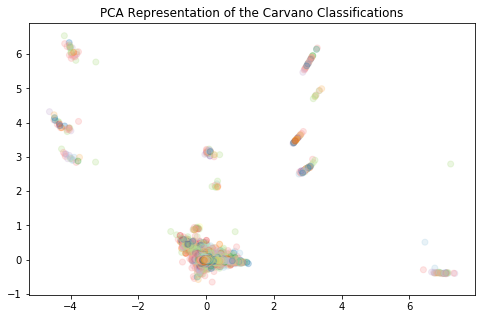
\includegraphics[width=0.45\textwidth]{images/carvano_pca.png}
\label{fig:carvano_pca}}
\hfil
\subfloat[TSNE Reduction]{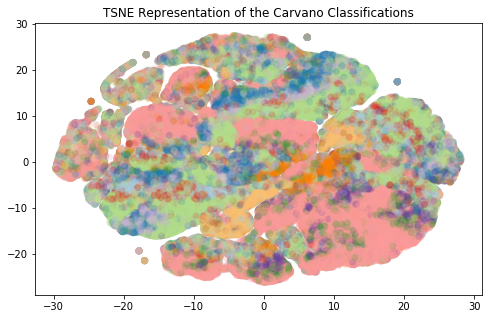
\includegraphics[width=0.45\textwidth]{images/carvano_tsne.png}
\label{fig:carvano_tsne}}
\caption{Dimensionality Reduction of Carvano's UGRIZ-based Classifications}
\label{fig:carvano}
\end{figure*}

\begin{figure*}[H]
\centering
\subfloat[PCA Reduction]{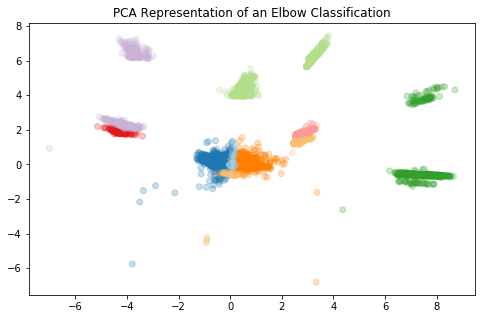
\includegraphics[width=0.45\textwidth]{images/elbow_pca.png}
\label{fig:elbow_eq_pca}}
\hfil
\subfloat[TSNE Reduction]{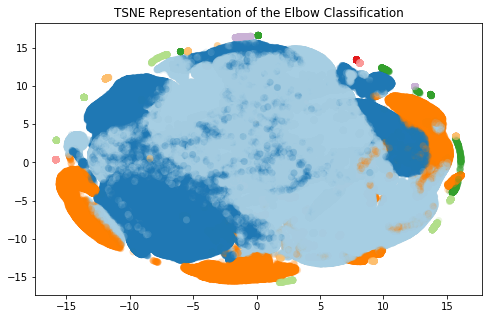
\includegraphics[width=0.45\textwidth]{images/elbow_tsne.png}
\label{fig:elbow_eq_tsne}}
\caption{Dimensionality Reduction of the Equation-Based Elbow Method with K-Means++}
\label{fig:elbow_eq}
\end{figure*}

\begin{figure*}[H]
\centering
\subfloat[PCA Reduction]{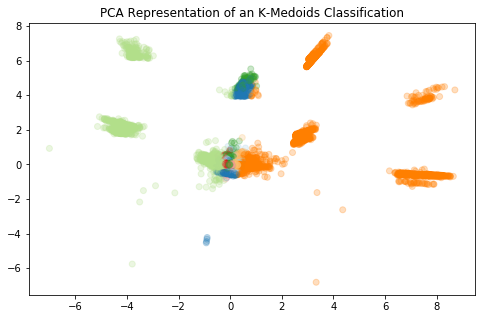
\includegraphics[width=0.45\textwidth]{images/kmed_pca.png}
\label{fig:kmed_pca}}
\hfil
\subfloat[TSNE Reduction]{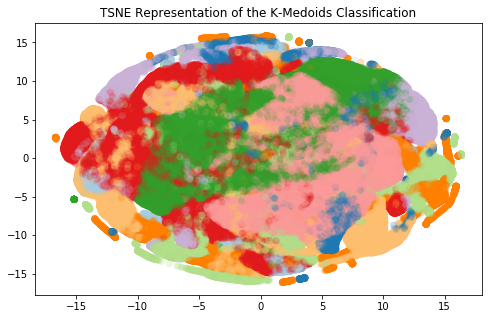
\includegraphics[width=0.45\textwidth]{images/kmed_tsne.png}
\label{fig:kmed_tsne}}
\caption{Dimensionality Reduction of K-Medoids Clustering}
\label{fig:kmed}
\end{figure*}

\begin{figure*}[H]
\centering
\subfloat[Graphical K-Means++ Elbow Method]{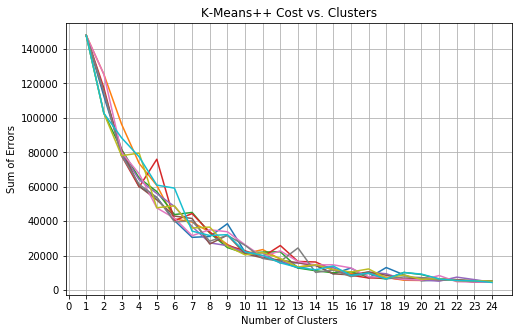
\includegraphics[width=0.5\textwidth]{kmeans-elbow}%
\label{fig:elbow}}
\hfil
\subfloat[K-Medoids Cluster Selection]{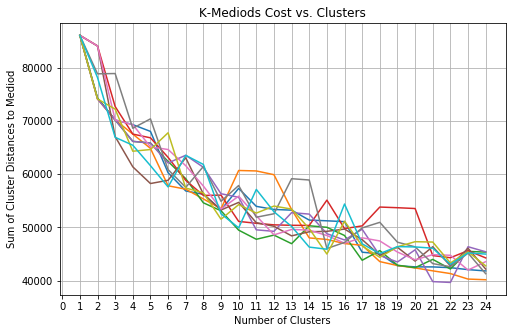
\includegraphics[width=0.5\textwidth]{kmed-cost}%
\label{fig:kmed_cost}}
\caption{Cost/Error Analysis for the K-Means++ Elbow Method, K-Medoids Cluster Selection.}
\label{fig:costs}
\end{figure*}

\begin{figure*}[ht]
\centering
\subfloat[PCA Reduction of HDBSCAN*]{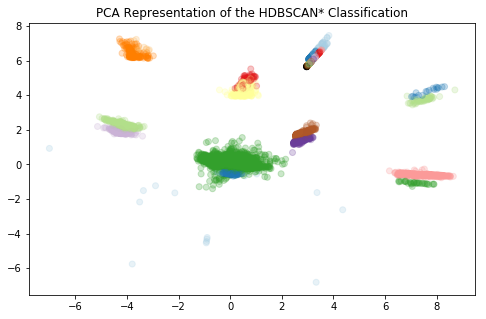
\includegraphics[width=0.45\textwidth]{images/hdbscan_pca.png}
\label{fig:hdbscan_pca}}
\hfil
\subfloat[PCA Reduction of Agglomerative Clustering]{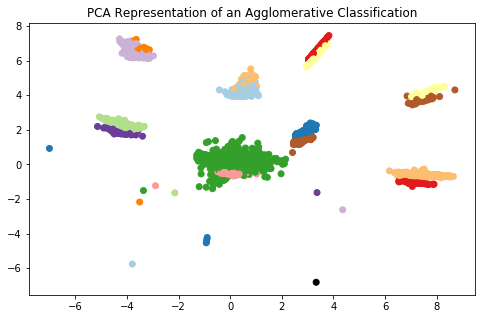
\includegraphics[width=0.45\textwidth]{images/agglomerative_pca.png}
\label{fig:agglomerative_tsne}}
\caption{Dimensionality Reduction of the Equation-Based Elbow Method with K-Means++}
\label{fig:hdb_agg}
\end{figure*}

\begin{figure*}[ht]
\centering
\subfloat{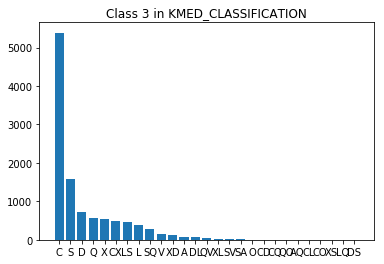
\includegraphics[width=0.45\textwidth]{images/bar-sample.png}
\label{fig:bar_1}}
\hfil
\subfloat[]{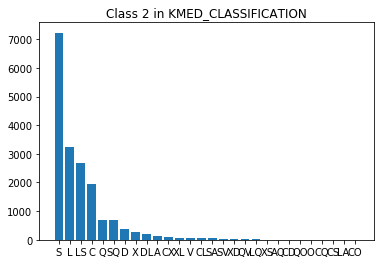
\includegraphics[width=0.45\textwidth]{images/bar-sample-2.png}
\label{fig:bar_2}}
\caption{Sample bar Graphs Against Carvano with K-Medoids}
\label{fig:bar}
\end{figure*}
% that's all folks
\end{document}
